% Figure 2: Phi-Scaled Vibrational Eigenmodes
% Energy level diagram with golden ratio (φ = 1.618) spacing
\documentclass[tikz,border=5pt]{standalone}
\usepackage{tikz}
\usetikzlibrary{calc,decorations.pathmorphing,arrows.meta}

\begin{document}
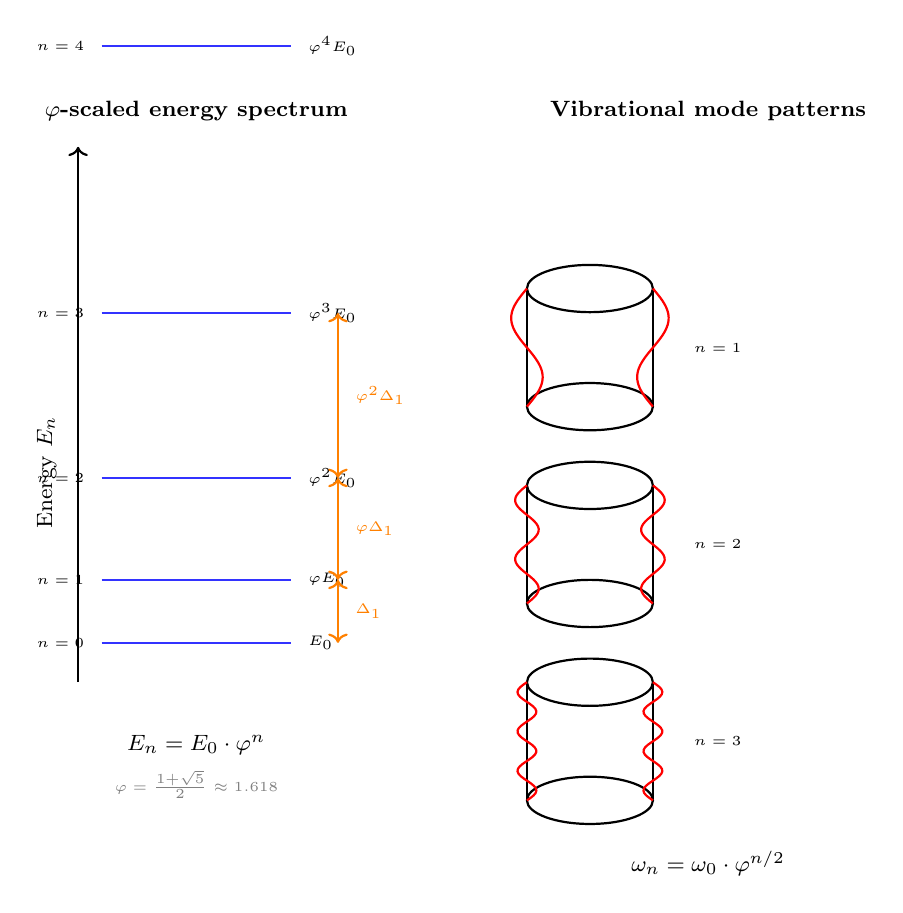
\begin{tikzpicture}[scale=1]

% === Define golden ratio ===
\pgfmathsetmacro{\phi}{1.618}

% === LEFT PANEL: Energy Level Diagram ===
\begin{scope}[shift={(-3.5,0)}]
    % Title
    \node[above,font=\footnotesize\bfseries] at (1.5,7) {$\varphi$-scaled energy spectrum};

    % Vertical axis
    \draw[->,thick] (0,0) -- (0,6.8);
    \node[left,font=\footnotesize,rotate=90] at (-0.4,3.5) {Energy $E_n$};

    % Energy levels with phi scaling
    % E_n proportional to phi^n
    \pgfmathsetmacro{\escale}{0.8}

    % Ground state n=0
    \pgfmathsetmacro{\Ezero}{0.5}
    \draw[thick,blue!80] (0.3,\Ezero) -- (2.7,\Ezero);
    \node[left,font=\tiny] at (0.2,\Ezero) {$n=0$};
    \node[right,font=\tiny] at (2.8,\Ezero) {$E_0$};

    % n=1
    \pgfmathsetmacro{\Eone}{\Ezero + \escale*1}
    \draw[thick,blue!80] (0.3,\Eone) -- (2.7,\Eone);
    \node[left,font=\tiny] at (0.2,\Eone) {$n=1$};
    \node[right,font=\tiny] at (2.8,\Eone) {$\varphi E_0$};

    % n=2
    \pgfmathsetmacro{\Etwo}{\Ezero + \escale*(1+\phi)}
    \draw[thick,blue!80] (0.3,\Etwo) -- (2.7,\Etwo);
    \node[left,font=\tiny] at (0.2,\Etwo) {$n=2$};
    \node[right,font=\tiny] at (2.8,\Etwo) {$\varphi^2 E_0$};

    % n=3
    \pgfmathsetmacro{\Ethree}{\Ezero + \escale*(1+\phi+\phi*\phi)}
    \draw[thick,blue!80] (0.3,\Ethree) -- (2.7,\Ethree);
    \node[left,font=\tiny] at (0.2,\Ethree) {$n=3$};
    \node[right,font=\tiny] at (2.8,\Ethree) {$\varphi^3 E_0$};

    % n=4
    \pgfmathsetmacro{\Efour}{\Ezero + \escale*(1+\phi+\phi*\phi+\phi*\phi*\phi)}
    \draw[thick,blue!80] (0.3,\Efour) -- (2.7,\Efour);
    \node[left,font=\tiny] at (0.2,\Efour) {$n=4$};
    \node[right,font=\tiny] at (2.8,\Efour) {$\varphi^4 E_0$};

    % Spacing annotations (show phi ratio)
    \draw[<->,orange,thick] (3.3,\Ezero) -- (3.3,\Eone);
    \node[right,font=\tiny,orange] at (3.4,{(\Ezero+\Eone)/2}) {$\Delta_1$};

    \draw[<->,orange,thick] (3.3,\Eone) -- (3.3,\Etwo);
    \node[right,font=\tiny,orange] at (3.4,{(\Eone+\Etwo)/2}) {$\varphi\Delta_1$};

    \draw[<->,orange,thick] (3.3,\Etwo) -- (3.3,\Ethree);
    \node[right,font=\tiny,orange] at (3.4,{(\Etwo+\Ethree)/2}) {$\varphi^2\Delta_1$};

    % Equation
    \node[font=\footnotesize] at (1.5,-0.8) {$E_n = E_0 \cdot \varphi^n$};
    \node[font=\tiny,gray] at (1.5,-1.3) {$\varphi = \frac{1+\sqrt{5}}{2} \approx 1.618$};
\end{scope}

% === RIGHT PANEL: Mode shapes on cylinder ===
\begin{scope}[shift={(3,0)}]
    % Title
    \node[above,font=\footnotesize\bfseries] at (1.5,7) {Vibrational mode patterns};

    % Mode n=1 (fundamental)
    \begin{scope}[shift={(0,5)}]
        \draw[thick] (0,0) ellipse (0.8 and 0.3);
        \draw[thick] (-0.8,0) -- (-0.8,-1.5);
        \draw[thick] (0.8,0) -- (0.8,-1.5);
        \draw[thick] (0,-1.5) ellipse (0.8 and 0.3);
        % Mode shape
        \draw[red,thick,domain=0:1.5,samples=50] plot ({0.8+0.2*sin(360*\x/1.5)},{-\x});
        \draw[red,thick,domain=0:1.5,samples=50] plot ({-0.8-0.2*sin(360*\x/1.5)},{-\x});
        \node[right,font=\tiny] at (1.2,-0.75) {$n=1$};
    \end{scope}

    % Mode n=2
    \begin{scope}[shift={(0,2.5)}]
        \draw[thick] (0,0) ellipse (0.8 and 0.3);
        \draw[thick] (-0.8,0) -- (-0.8,-1.5);
        \draw[thick] (0.8,0) -- (0.8,-1.5);
        \draw[thick] (0,-1.5) ellipse (0.8 and 0.3);
        % Mode shape (2 nodes)
        \draw[red,thick,domain=0:1.5,samples=50] plot ({0.8+0.15*sin(720*\x/1.5)},{-\x});
        \draw[red,thick,domain=0:1.5,samples=50] plot ({-0.8-0.15*sin(720*\x/1.5)},{-\x});
        \node[right,font=\tiny] at (1.2,-0.75) {$n=2$};
    \end{scope}

    % Mode n=3
    \begin{scope}[shift={(0,0)}]
        \draw[thick] (0,0) ellipse (0.8 and 0.3);
        \draw[thick] (-0.8,0) -- (-0.8,-1.5);
        \draw[thick] (0.8,0) -- (0.8,-1.5);
        \draw[thick] (0,-1.5) ellipse (0.8 and 0.3);
        % Mode shape (3 nodes)
        \draw[red,thick,domain=0:1.5,samples=50] plot ({0.8+0.12*sin(1080*\x/1.5)},{-\x});
        \draw[red,thick,domain=0:1.5,samples=50] plot ({-0.8-0.12*sin(1080*\x/1.5)},{-\x});
        \node[right,font=\tiny] at (1.2,-0.75) {$n=3$};
    \end{scope}

    % Frequency relation
    \node[font=\footnotesize] at (1.5,-2.3) {$\omega_n = \omega_0 \cdot \varphi^{n/2}$};
\end{scope}

\end{tikzpicture}
\end{document}
